% -----------------------------------------------
% Template for JIM
%     jim.sty -> style file
% By Eloi Batlle (eloi@iua.upf.es), changes for 
% ICMC by Bram de Jong (bdejong@iua.upf.es)
% changes for JIM 2007 by Dominique Fober (fober@grame.fr)
% changes for JIM 2009 by Olivier Tache (olivier.tache@imag.fr)
% -----------------------------------------------

\documentclass{article}
\usepackage{jim,amsmath}
\usepackage[utf8]{inputenc}
\usepackage[francais]{babel}
\usepackage[T1]{fontenc}
\usepackage{enumitem}
\usepackage{graphicx}
\usepackage{balance}
\usepackage{ifpdf}
\usepackage{hyperref}
\usepackage{amssymb,amsmath} 
\usepackage{verbatim}
\usepackage{color}
\usepackage{float}

\definecolor{mygrey}{gray}{0.95}

\newcommand{\OSC}[1]	{{\fontsize{9pt}{9pt} \selectfont\texttt{#1}}}
\newcommand{\note}[1]	{\textcolor{red}{(#1)}}

\newcommand{\lowTilde}{\texttildelow}
\newcommand{\tab}{\hspace*{4mm}}
\let\olditemize\itemize
\let\oldenditemize\enditemize
\renewenvironment{itemize} 	{\olditemize \renewcommand{\labelitemi}{$\bullet$} \setlength{\itemsep}{0mm}}{\oldenditemize}

\newcommand{\sample}[1]		{\vspace{-0.2em}\begin{center}\colorbox{mygrey}{\begin{minipage}[t]{0.98\columnwidth} {\small \texttt{#1}}\end{minipage}}\end{center}}


% Title.
% ------
\title{Le modèle du temps dans INScore.}

% Single \textsc{address}
% To use with only one author or several with the same address
% ---------------
\oneauthor
  {D. Fober \quad Y. Orlarey \quad S. Letz} {Grame \\
  Centre nationale de création musicale \\
  Lyon - France \\
     {\tt {\small \{fober, orlarey, letz\}@grame.fr}}}

% Two addresses
% --------------
%\twoauthors
%  {First author} {School \\ Department}
%  {Second author} {Company \\ Address}

% Three addresses
% --------------
%\threeauthors
%  {Auteur 1} {Organisme \\ Adresse électronique}
%  {Auteur 2} {Organisme \\ Adresse électronique}
%  {Auteur 3} {Organisme \\ Adresse électronique}

\begin{document}
%
\maketitle
%
\begin{abstract}
INScore est un environnement pour la conception de partition interactives augmentées, tourné vers des usages non conventionnels de la notation musicale, sans exclure pour autant les approches classiques. Dans cet environnement, bien que tous les objets de la partition aient une dimension temporelle, le temps reste \emph{fixe} i.e. que la date (ou la durée) d'un objet ne change pas, sauf à réception d'un message qui ne peut être produit que de manière externe ou événementielle. INScore n'inclut donc pas de gestionnaire du temps au sens classique du terme. 
A l'origine, ce choix a été dicté par le fait que le système fut conçu pour des usages couplés avec des logiciels de production sonore (e.g. Max/MSP, Pure Data), qui ont des contraintes de temps-réel plus strictes que l'environnement graphique d'INScore.
Toutefois, la nécessité d'introduire un temps dynamique a progressivement émergé, conduisant à un modèle original, à la fois \emph{événementiel} et continu. C'est ce modèle qui est présenté et ses propriétés dans l'environnement d'INScore.
\end{abstract}

%==============================================================
\section{Introduction}\label{sec:introduction}

Les manipulations du temps dans les environnements pour la composition musicale peuvent s'exprimer de manière très différentes.

Dans Open Music, il y a 3 principaux types d'expression du temps: "le temps musical (i.e. le temps de la notation symbolique, relatif à un tempo), le temps proportionnel (exprimé en millisecondes) et le temps continu (défini par des fonctions mathématiques)"~\cite{bresson08}. 

Dans d'autres environnements comme Antescofo \cite{acont08} ou iScore \cite{AllombertDA08}, le temps est également \textit{événementiel} et peut notamment se décrire en terme de relations de Allen \cite{Allen:1983:MKT:182.358434}, ce qui permet d'introduire des aspects réactifs dans les oeuvres. 
Plus récement, ces aspects réactifs ont été également introduits dans Open Music \cite{bresson:hal-00965747}, témoignant de leur importance dans les approches compositionnelles contemporaines.

Le temps dans INScore \cite{Fober:12a} est \emph{fixe} : tous les objets possèdent une date et une durée exprimée en temps musical qui sont fixés dans la description de la partition. La dimension temporelle commune des objets d'une partition  permet de représenter leurs relations temporelles dans l'espace graphique \cite{fober:10b}. L'\emph{animation} du temps (i.e. la modification des attributs temporel d'un objet) se fait à la réception de messages OSC, nécessairement émis depuis une application externe.

Ce choix initial d'un temps \emph{fixe} a été dicté par une conception orientée vers des usages couplés avec des logiciels de production sonore (e.g. Max/MSP, Pure Data), qui ont des contraintes de temps-réel strictes et de ce fait, offrent des mécanismes de gestion du temps efficaces et précis. Néanmoins, les aspects réactifs ont été rapidement pris en compte avec l'introduction d'\textit{événements} qui permettent d'interagir avec la partition \cite{fober13a}. Initialement, la typologie de ces événements inclus des interactions classiques de type "interface utilisateur" (e.g. interactions avec la souris), et introduit des événements dans le domaine temporel avec notamment la \textit{surveillance} d'intervalles temporels. Ce mécanisme d'\textit{événements} a ouvert la voie à une approche originale de la programmation de partitions en offrant à l'utilisateur, la possibilité de placer des messages - et donc des interactions - dans l'espace temporel. Il n'en demeurait pas moins que le temps étant toujours \emph{fixe}, l'usage d'une application externe restait nécessaire pour l'actionner.

La nécessité d'un temps \emph{dynamique} a de ce fait émergé. Elle a été résolue de manière simple, avec l'introduction d'un attribut supplémentaire aux objets d'une partition : le \emph{tempo}. Ce simple ajout a néanmoins un impact important sur la conception du temps dans INScore et sur les aspects dynamiques des partitions. Nous présenterons tout d'abord le modèle du temps musical, qui est contrôlé par le tempo. Nous verrons ensuite comment ce temps se combine avec le temps événementiel, et permet de programmer des partitions dynamiques \emph{autonomes}. Nous montrerons enfin quelques cas d'utilisation avant de conclure et de donner quelques perspectives pour l'extension des dimensions temporelles des objets de la partition.


%==============================================================
\section{Le modèle du temps musical}\label{mustime}

Du point de vue utilisateur et pour un objet donné, le temps est actif quand son attribut tempo est non nul : une valeur non nulle du tempo a pour effet de déplacer l'objet dans le temps musical, en fonction de son tempo et de l'écoulement du temps absolu. \\
Nous parlerons de \emph{date} pour faire référence au temps musical d'un objet, et de \emph{moment} pour faire référence à un point dans l'écoulement du temps absolu. \\

Soit $t_0$, le moment d'activation du temps d'un objet et $v$ la valeur de son tempo, la date $d_t$ de l'objet à un instant $t$ est donnée par une fonction du temps $f$ telle que :
\begin{equation}
%\[
	 f(t) \to d_t = d_t{_0} + (t - t_0) \times v \times k , \quad t \geqq t_0
%\]
\label{timeeq}
\end{equation}
où $d_i$ est la date de l'objet au moment $t_i$ et $k$ une constante permettant de convertir le temps absolu en temps musical. Dans la pratique, le temps absolu est exprimé en millisecondes et l'unité de temps musical est la ronde. De ce fait, la valeur de la constante $k$ est $1 / 1000 \times 60 \times 4$.

Chaque objet de la partition a un tempo indépendant. La valeur du tempo est signée, ce qui signifie qu'un objet peut se déplacer dans tous les sens du temps (en avant ou en arrière). Il y a peu d'environnement permettent d'exprimer ce renversement du temps de manière simple et naturelle, de ce point de vue on peut citer IanniX \cite{iannix14}, un séquenceur graphique inspiré des travaux de Iannis Xenakis et que l'on peut voir comme un système d'écriture du temps.

%=======================================
\subsection{Implémentation}

Dans INScore, la granularité du temps est celle de l'affichage : le système fonctionne de manière asynchrone et une tâche du temps périodique traite les messages entrants et calcule le rendu graphique. Dans la pratique, comme les effets du temps ne sont visibles que dans l'espace graphique, nous considérons qu'il n'est pas nécessaire d'adopter une granularité plus fine. 

Par ailleurs, la fréquence de la tâche du temps peut être variable : 
\begin{itemize}
\item par défaut, elle est effectuée toutes les 10 mls mais l'utilisateur peut changer librement cette valeur en adressant le message \OSC{rate} à l'application, suivi d'une valeur en millisecondes.
\item cette tâche n'est pas réentrante et la complexité de l'affichage peut potentiellement la ralentir.
\end{itemize}
De ce fait et à chaque tâche du temps, le système mesure le temps réellement écoulé. Les objets dont le tempo n'est pas nul utilisent alors cette valeur pour calculer un offset en temps musical comme indiqué en (\ref{timeeq}), puis s'auto-envoient un message \OSC{ddate} (déplacement de la date en mode relatif) avec la valeur correspondante.

\begin{figure}[h]
   \centering
   \sample{/ITL/scene/obj tempo 60 \\
   \\
-> /ITL/scene/obj ddate $f(r_i)$ \\
-> /ITL/scene/obj ddate $f(r_{i+1})$ \\
-> /ITL/scene/obj ddate $f(r_{i+2})$ \\
-> ...
}
   \caption{Une séquence de messages qui activent le temps d'un objet \OSC{obj}. Les messages préfixés par \OSC{->} sont générés par l'objet lui même. $r_{i}$ représente la valeur du temps écoulé entre la tâche $i$ et $i-1$.}
   \label{fig:tempo}
\end{figure}

Pour être consistante avec l'ensemble du système, cette implémentation est entièrement basée sur des messages. De ce fait, elle est compatible avec tous les mécanismes d'INScore, tels que par exemple, le système de \emph{forwarding} des messages. 


%==============================================================
\section{Le temps événementiel}\label{evtime}

L'approche \emph{événementielle} du temps dans INScore a précédé le modèle du temps musical et a été présentée en \cite{fober13a}. Pour rappel, le processus d'interaction événementielle repose sur l'association de messages à des événements du système. Ces messages sont émis lorsque l'événement auquel ils sont associés se produit. Le format général des messages pour créer de telles associations est décrit en figure \ref{fig:watch}.

\begin{figure}[htbp]
\centerline{
	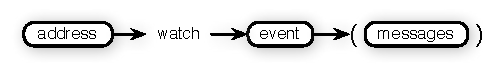
\includegraphics[width=0.95\columnwidth]{imgs/watch}}
\caption{Format général d'un message d'interaction : le message \OSC{watch} installe une liste de messages associés à l'événement \OSC{event}.}
\label{fig:watch}
\end{figure}


Dans la première version présentée, la typologie des événements était limitée à des événements classiques d'interface utilisateur (tels que clics de souris), étendus dans le domaine temporel (voir table \ref{tbl:evts}). 

\begin{table}[htp]
\begin{center}
\begin{tabular}{c|c}
Domaine graphique & Domaine temporel \\
\hline
mouseDown 		& timeEnter	\\
mouseUp			& timeLeave	\\
mouseEnter		& durEnter		\\
mouseLeave		& durLeave		\\
mouseMove		&				\\
\end{tabular}
\end{center}
\caption{Principaux événements du système dans sa version intiale.}
\label{tbl:evts}
\end{table}%

Cette typologie a été largement étendue pour inclure :
\begin{itemize}
\item n'importe quel attribut d'un objet : la modification de la valeur d'un attribut est potentiellement génératrice de l'événement correspondant, qui porte le nom de l'attribut (e.g. \OSC{x, y date}, etc.). 
\item les données intrinsèques d'un objet i.e. fixées par un message \OSC{set}. Il s'agit de l'événement \OSC{newData}, introduit pour les besoins de la composition de partitions symboliques \cite{lepetit16}.
\item des événements arbitraires définis par l'utilisateur.
\end{itemize}
\vspace*{1mm}
Tout événement peut être arbitrairement déclenché avec l'émission d'un message \OSC{event} suivi de ses paramètres. Conceptuellement, ce message \OSC{event} est équivalent à l'appel d'une fonction paramétrée, et génère des messages OSC en sortie. 
Cette logique est particulièrement consistante pour les événements utilisateurs, qui peuvent prendre un nombre variable de paramètres, ceux-ci étant ensuite accessibles dans les messages associés sous la forme de variables nommées $\$1...\$n$. La figure \ref{fig:uevent} présente un ex-emple d'événement utilisateur à 2 arguments.

\begin{figure}[h]
   \centering
   \sample{/ITL/scene/obj watch MYEVENT ( \\
\tab/ITL/scene/t1 set txt \$1, \\
\tab/ITL/scene/t2 set txt \$2 \\
);   \\   
/ITL/scene/obj event MYEVENT \\
\hspace*{25mm}"This text is for t1"\\
\hspace*{25mm}"This one is for t2"; 
}
   \caption{Définition d'un événement utilisateur nommé \OSC{MYEVENT} qui attend 2 paramètres référencés par \$1 et \$2. Cet événement est ensuite déclenché avec 2 chaines de caractères comme arguments.}
   \label{fig:uevent}
\end{figure}


La dimension temporelle de cette logique \emph{événementielle} permet de placer des \emph{fonctions} dans l'espace temporel, sous forme d'événements qui activent des listes de messages pouvant modifier l'état du système et/ou s'adresser à des applications externes via l'adressage OSC étendu. La figure \ref{fig:events} en donne un exemple.
  
\begin{figure}[h]
   \centering
   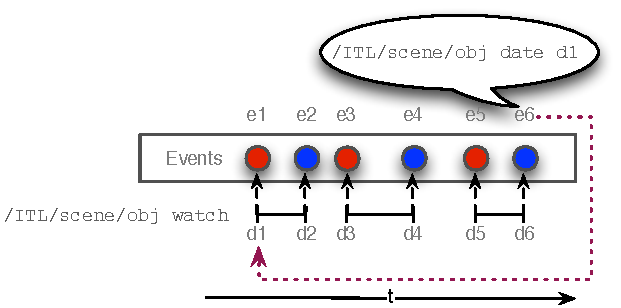
\includegraphics[width=0.95\columnwidth]{imgs/events}
   \caption{Exemple d'événements placés dans l'espace temporel pour un objet \OSC{obj}. Ces événements sont associés à des intervalles de temps (\OSC{timeEnter} et \OSC{timeLeave}) et sont déclenchés à l'entrée (en rouge) ou à la sortie (en bleu) de ces intervalles. Le dernier événement (\OSC{e6}), émet un message \OSC{date} qui crée une boucle en renvoyant l'objet au début du premier intervalle.}
   \label{fig:events}
\end{figure}

%==============================================================
\subsection{Implémentation}

Chaque objet de la partition gère des relations entre un ensemble d'événements $\mathbb{E}$ et un ensemble de listes de messages $\mathbb{M}$. L'ensemble des événements $\mathbb{E}_o$ d'un objet $o$ est un ensemble polymorphe défini comme : 
\[
	\mathbb{E}_o = \mathbb{A}_o \cup \mathbb{U}_o \cup \mathbb{T}_o \cup \mathbb{T'}_o \cup \mathbb{K}  
\] 
où :
\begin{itemize}
\item[-] $\mathbb{A}_o$ est l'ensemble des attributs de l'objet $o$, 
\item[-] $\mathbb{U}_o$ est l'ensemble des événements utilisateur de l'objet $o$, 
\item[-] $\mathbb{T}_o$ et $\mathbb{T'}_o$ sont respectivement l'ensemble des intervalles temporels surveillés en entrée et en sortie,
\item[-] $\mathbb{K}$ est l'ensemble des événements associés à l'interface utilisateur (\OSC{mousexxx, touchxxx}).
\end{itemize}
L'ensemble $\mathbb{K}$ est indépendant de l'objet $o$ alors que l'ensemble $\mathbb{A}$ dépend de ses attributs et que les ensembles $\mathbb{U}$, $\mathbb{T}$ et $\mathbb{T'}$ sont dynamiques (vides par défaut).

Un événement $e$ sera dit déclencheur quand:
\[
	\exists (e, m) \in \mathbb{E}_o \times \mathbb{M}_o  
\] 
Les messages de $m$ sont alors envoyés.

Le calcul d'un événement $e$ est dépendant du type de l'événement:
\begin{itemize}
\item[-] pour un message $x$ adressé à un objet $o$, un événement sera émis si $x \in \mathbb{A}_o$, 
\item[-] pour un message \OSC{event x} adressé à un objet $o$, un événement sera émis si $x \in \mathbb{U}_o \cup \mathbb{A}_o \cup  \mathbb{K}$,
\item[-] pour un message \OSC{date x} addressé à un objet $o$ qui porte la date $d$, un événement sera émis si :\\ 
\hspace*{3.5mm} $\exists i \in \mathbb{T}_o\ \ |\ (x \in i\ \land\ d \not\in i)$ \\
ou $\exists i \in \mathbb{T'}_o\ |\ (x \not \in i\ \land\ d \in i)$,
\item[-] les événements de $\mathbb{K}$ sont calculés par le système hôte.
\end{itemize}


%==============================================================
\section{Partitions dynamiques}

La combinaison du temps musical et événementiel permet de concevoir des partitions dynamiques autonomes. Dans l'exemple suivant 3 objets \OSC{o1, o2} et \OSC{o3} s'activent mutuellement (figure \ref{fig:ex1}) selon le schéma temporel décrit par la figure \ref{fig:sample}. Il fait usage des 2 événements \emph{utilisateur} \OSC{START} et \OSC{STOP}. Ceux-ci sont décrits en figure \ref{fig:ex2}.

\begin{figure}[h]
   \centering
\sample{/ITL/scene/o1 watch timeLeave 0 \$t2 \\
   \tab( /ITL/scene/o2 event START );\\
	/ITL/scene/o1 watch timeLeave 0 \$d1 \\
	\tab( /ITL/scene/o1 event STOP );\\
	/ITL/scene/o2 watch timeLeave 0 \$d2 \\
	\tab( /ITL/scene/o2 event STOP, \\
	\tab \tab/ITL/scene/o3 event START );\\
	/ITL/scene/o3 watch timeLeave 0 \$d3 \\
	\tab( /ITL/scene/o3 event STOP, \\
	\tab \tab/ITL/scene/o1 event START );
}
   \caption{Activation mutuelle de 3 objets \OSC{o1, o2, o3} selon un schéma temporel prédéfini.}
   \label{fig:ex1}
\end{figure}

Les variables \OSC{\$t1, \$d1, \$d2} et \OSC{\$d3} sont instanciées avec des valeurs correspondant à la figure \ref{fig:sample}. On notera que l'objet \OSC{o3} boucle l'ensemble du système en activant l'événement \OSC{START} de l'objet \OSC{o1}.

\begin{figure}[h]
   \centering
\sample{/ITL/scene/o* watch STOP ( \\
   \tab/ITL/scene/\$self tempo 0,\\
   \tab/ITL/scene/\$self alpha \$alpha	\\
);\\
\\
/ITL/scene/o* watch START ( \\
   \tab/ITL/scene/\$self tempo 120,\\
   \tab/ITL/scene/\$self alpha 255,\\
   \tab/ITL/scene/\$self date 0\\
);
}
   \caption{Définition des événements utilisateur \OSC{START} et \OSC{STOP}.}
   \label{fig:ex2}
\end{figure}


Les événements \OSC{START} et \OSC{STOP} activent et désactivent respectivement le temps de l'objet récepteur en changeant la valeur de son tempo, et en modifiant son aspect graphique (canal alpha) pour rendre compte de l'activation du temps. L'événement \OSC{START} positionne par ailleurs la date de l'objet à 0, ce qui permet le bouclage du système par \OSC{o3}.
\begin{figure}[h]
   \centering
   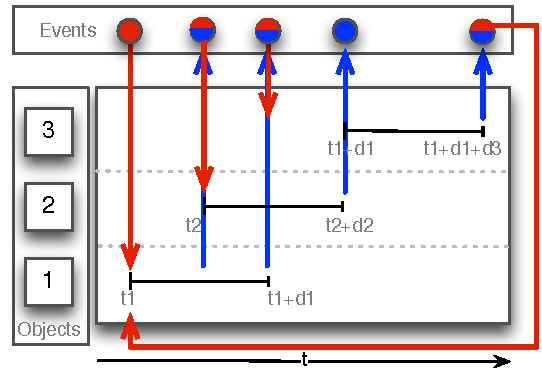
\includegraphics[width=0.8\columnwidth]{imgs/sample}
   \caption{Représentation de l'activation du temps pour 3 objets de la partition. La couleur rouge est utilisée pour les événements \OSC{START}, le bleu pour les événements \OSC{STOP}.}
   \label{fig:sample}
\end{figure}


%==============================================================
\subsection{Jeu est un autre}

\emph{Jeu est un autre} est une pièce pédagogique pour ordinateur et effectif variable de Vincent Carinola, où Max/MSP est mis en oeuvre pour calculer des processus sonores et activer une partition dynamique à l'intention des instrumentistes. 

La partition (figure \ref{fig:sample}) comprend un ensemble de figures munies de labels (sculpture, zébrure, allure, texture, tournure), reliées par des chemins. A chaque figure (que nous appelerons \emph{stations}) est associée un mode de jeu instrumental ainsi des processus sonores spécifiques, basés sur des matériaux préparés par les élèves. Par exemple, le chemin \emph{murmure} indique que \emph{le passage d'une figure à une autre se fait en traversant un chemin habité par des murmures. Il faut ici trouver, dans le jeu instrumental et vocal, ce qui s'apparenterait le plus à une histoire que l'on raconterait très doucement, en chuchotant.}\footnote{extrait des instructions données avec la partition.}.

Dans cette pièce, l'ordinateur joue en quelque sorte le rôle de chef d'orchestre : il calcule des séquences sonores basées sur les matériaux pré-enregistrés et active des chemins ou des stations pour des durées variables, calculées dynamiquement. Les chemins et stations possibles sont indiqués sur la figure \ref{fig:sample} par les labels P1 à P13. 

Les aspects dynamiques de la partition sont définis avec des événements utilisateurs qui portent le nom des labels correspondants. Ces événements prennent une durée en paramètre, de sorte que pour activer un chemin ou une station, il suffit d'émettre le message :\\
\tab \tab \OSC{/ITL/scene Px d} \\
où \OSC{Px} est le nom de l'événement (\OSC{P1...P13})\\
 et \OSC{d} la durée correspondante. \\
C'est donc une approche de haut niveau qui, du côté de Max/MSP, permet de \emph{conduire} la partition en temps réel.

\vspace{2mm}
Visuellement, la partition rend compte de ces événements dans l'espace graphique de deux manières :
\begin{itemize}
\item pour les stations (événements \OSC{P1...P4} et \OSC{P13}) : en utilisant le canal alpha de la figure correspondante pour indiquer son activation.
\item pour les chemins (événements \OSC{P5...P12}): en déplaçant un curseur le long du chemin, dans le sens correspondant.
\end{itemize}

Schématiquement, l'implémentation de ces événements repose sur un objet nommé \OSC{cursor} qui se déplace dans le temps à un tempo fixe, dépendant de l'unité de temps adoptée par Max/MSP. 

Pour les stations, elle consiste à changer le canal alpha de la figure correspondant, à activer le temps du curseur et à instancier un événement pour la fin de la durée calculée par Max/MSP (figure \ref{fig:station}). 
\begin{figure}[h]
   \centering
\sample{/ITL/scene watch P1 ( \\
\tab/ITL/scene/g1 alpha 255, \\
\tab/ITL/scene event STATION \$tempo '\$1' \\
); \\
\\
/ITL/scene watch STATION ( \\
\tab/ITL/scene/cursor show 0,\\
\tab/ITL/scene/cursor watch timeLeave \\
\hspace*{30mm}0 '\$2' \$stop\_s,\\
\tab/ITL/scene/cursor date 0,\\
\tab/ITL/scene/cursor tempo '\$1'\\
); \\
\\
stop\_s = ( \\
\tab\# set the tempo to 0 \\
\tab/ITL/scene/cursor tempo 0, \\
\tab\# remove any watched event \\
\tab/ITL/scene/cursor watch,  \\
\tab\# and reset the alpha channel \\
\tab/ITL/scene/g* alpha \$alpha \\
);
}
   \caption{Définition de l'événement \OSC{P1} qui active la station représentée par l'objet \OSC{g1}. A noter : l'utilisation de la variable \OSC{stop\_s}, qui est évaluée par le parser, et qui permet de partager le comportement d'arrêt entre plusieurs événements. Les variables \OSC{tempo} et \OSC{alpha} sont définies de manière globale.}
   \label{fig:station}
\end{figure}

Pour les chemins, la durée de l'arc correspondant est fixée à la durée de l'événement, le curseur est synchronisé sur cet arc en mode \OSC{syncframe} (qui consiste à synchroniser un objet sur la bordure d'un autre), son temps est activé et un événement est instancié pour la fin de la durée de l'arc (figure \ref{fig:chemin}).
\begin{figure}[h]
   \centering
\sample{/ITL/scene watch P5 ( \\
\tab/ITL/scene/a3 duration '\$1', \\
\tab/ITL/scene event CHEMIN a3 \$tempo '\$1' \\
); \\
\\
/ITL/scene watch CHEMIN ( \\
\tab/ITL/scene/cursor show 1,\\
\tab/ITL/scene/sync cursor '\$1' syncFrame,\\
\tab/ITL/scene/cursor watch timeLeave \\
\hspace*{30mm}0 '\$3' \$stop\_c,\\
\tab/ITL/scene/cursor date 0,\\
\tab/ITL/scene/cursor tempo '\$2'\\
); \\
\\
stop\_c = ( \\
\tab/ITL/scene/cursor show 0,\\
\tab/ITL/scene/cursor tempo 0, \\
\tab/ITL/scene/cursor watch,  \\
\tab\# remove the synchronization \\
\tab/ITL/scene/sync cursor \\
);
}
   \caption{Définition de l'événement \OSC{P5} qui active le chemin représenté par l'objet \OSC{a3}.}
   \label{fig:chemin}
\end{figure}



%==============================================================
\section{Conclusions}
L'approche temporelle proposée par INScore fournit un support original à la conception de partition dynamiques. Elle permet d'exprimer des comportements arbitraires à la fois dans le temps musical et événementiel.  
Elle reste toutefois limitée : à la différence d'environnements comme Antescofo par exemple, les événements n'ont pas de dimension temporelle ce qui interdit de les composer avec des opérations d'ordre logique. Il serait également intéressant d'étendre les dimensions temporelles d'un objet à tous ses attributs graphiques, de sorte que ses déplacements dans le temps puissent se traduire dans l'espace graphique par la variation de ses attributs.

\balance
\bibliographystyle{ieeetr}
\bibliography{../interlude}


\begin{figure*}[ht]
   \centering
   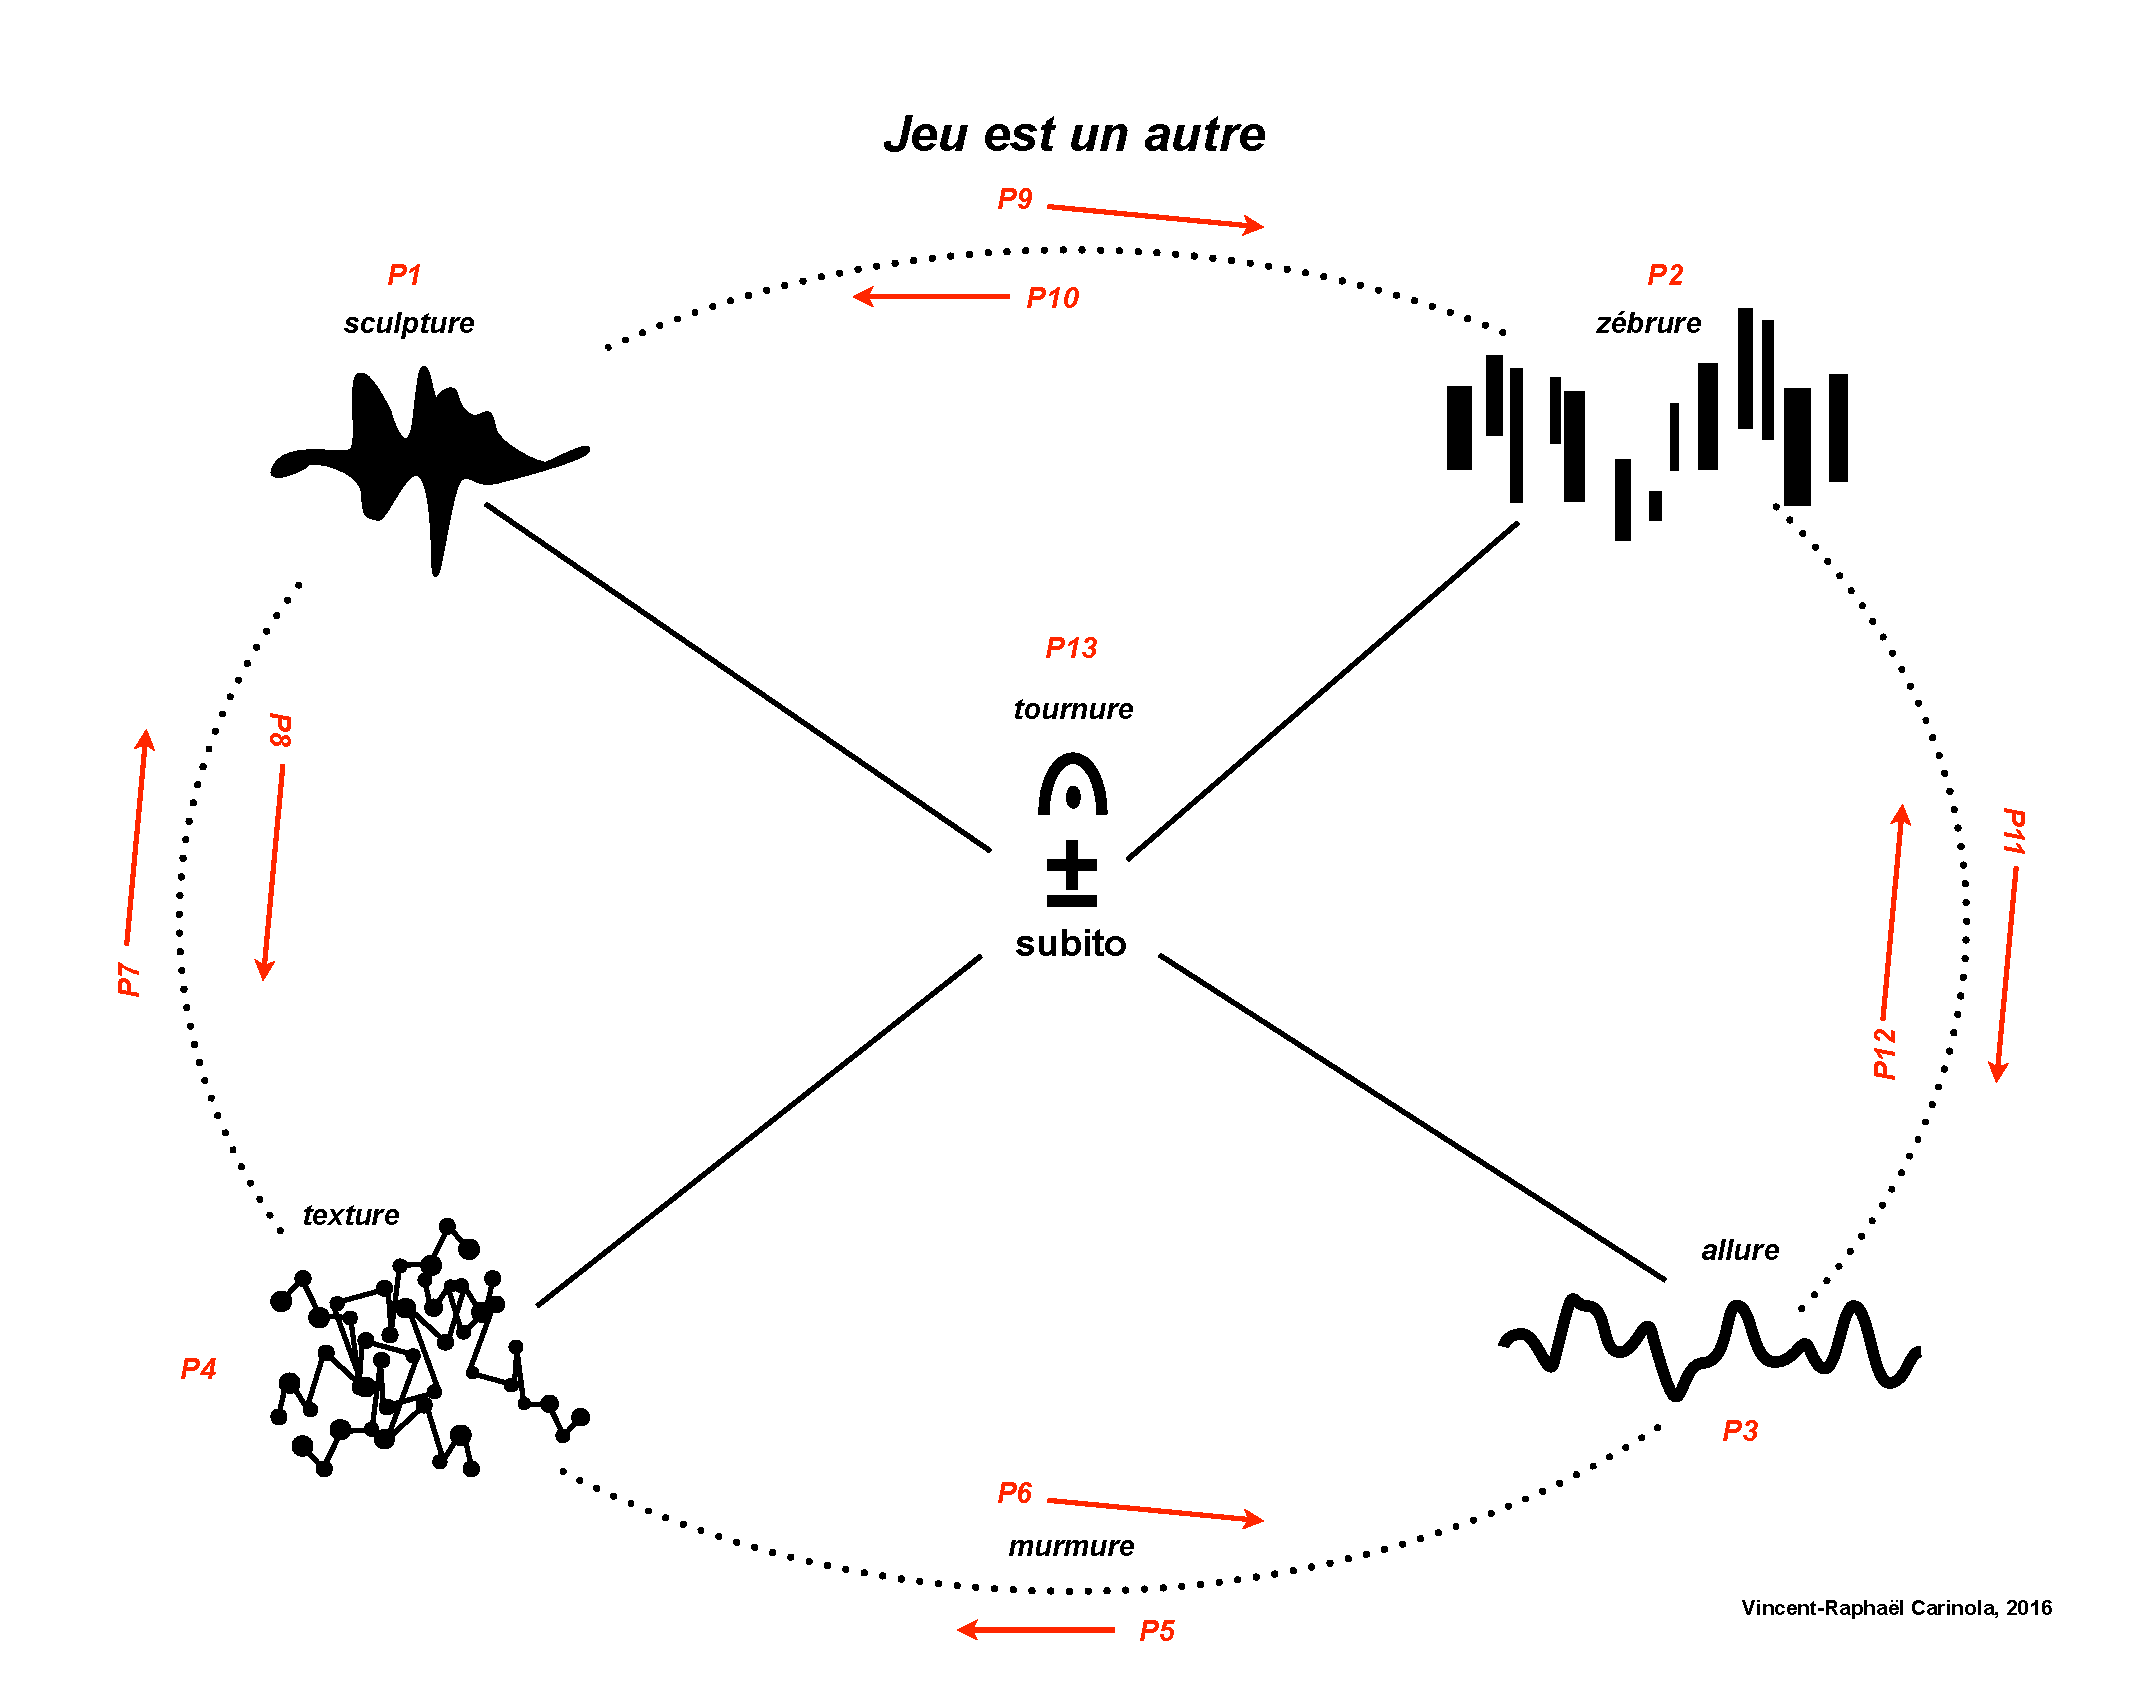
\includegraphics[width=0.8\textwidth]{imgs/jeu}
%   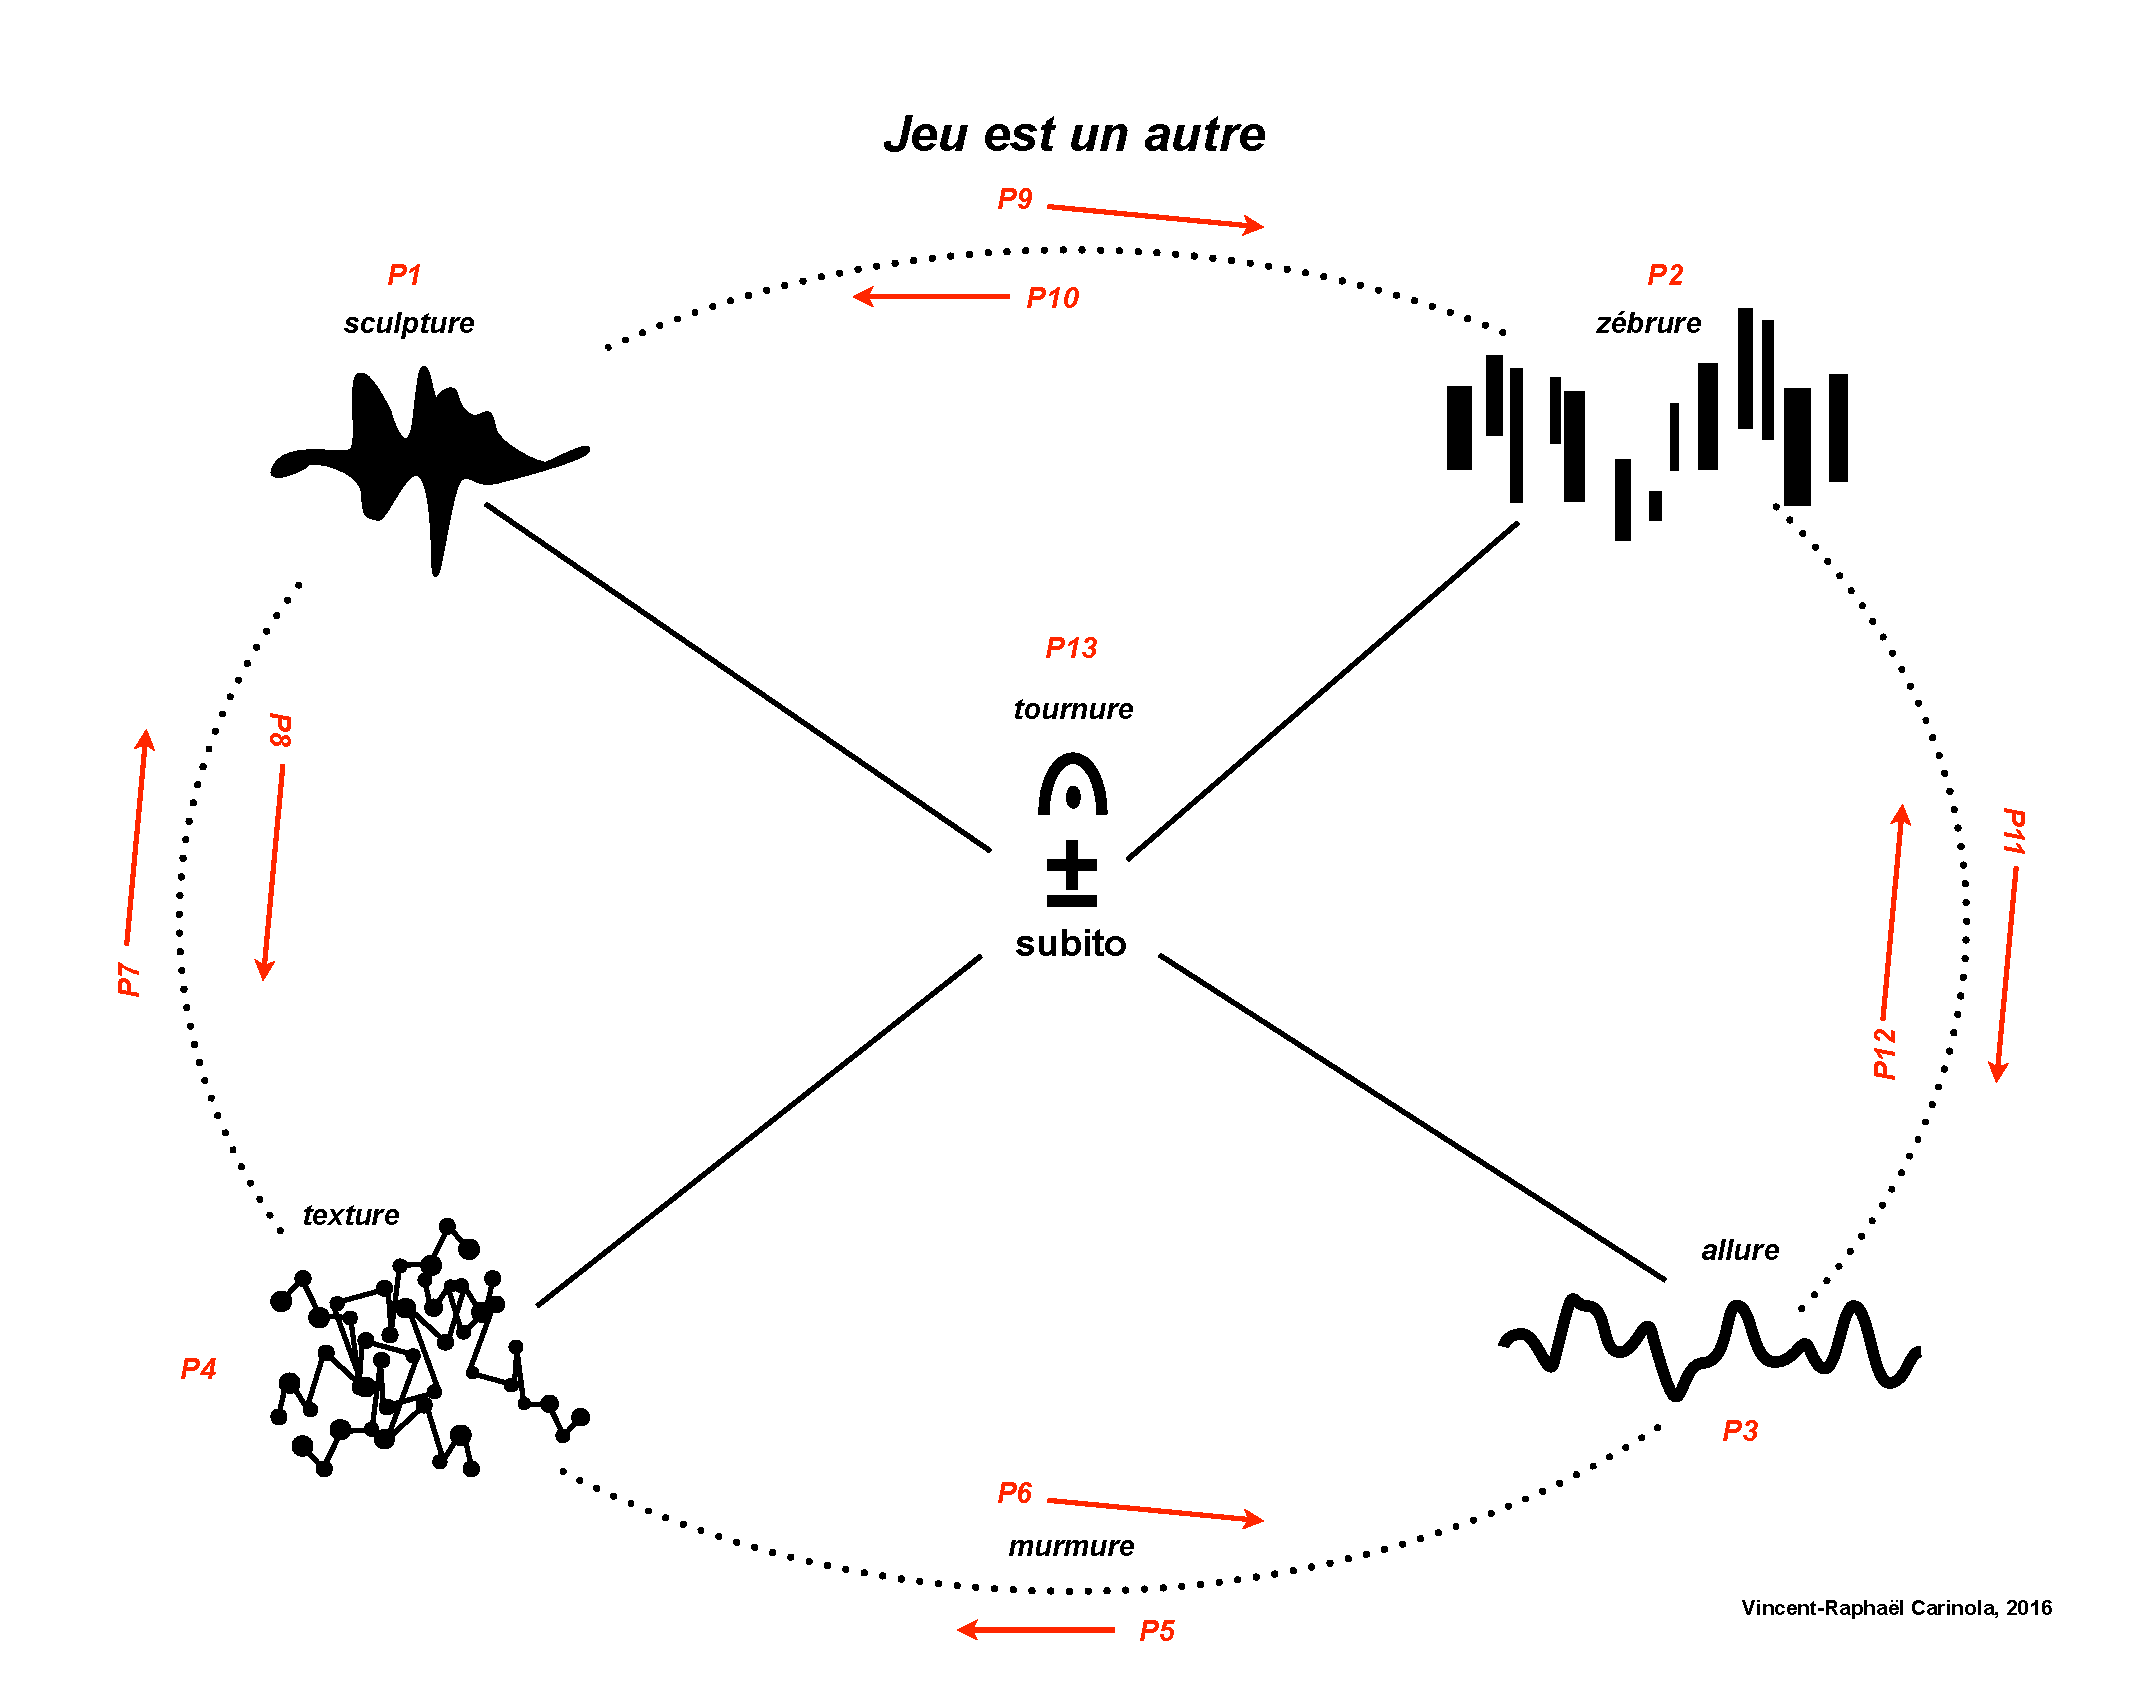
\includegraphics[width=1.0\columnwidth]{imgs/jeu}
   \caption{Partition de \emph{"Jeu est un autre"} annotée (en rouge) avec les chemins et les stations possibles. Ces annotations sont implémentées comme des événements utilisateur d'INScore, elles ne figurent pas sur la partition de l'instrumentiste.}
   \label{fig:sample}
\end{figure*}


\end{document}
